
% Spellcheck ok
% Mikes ok

\chapter{Two Variables: Establishing Relationships}{}{}
\label{ch:bivariate}

\index{data analysis!bivariate analysis|(}
\index{bivariate analysis|(}
  
\Fint{When we are dealing with a data set that consists of \emph{two}
variables (that is, a \emph{bivariate} data set),} we are mostly
interested in seeing whether some kind of relationship exists between
the two variables and, if so, what kind of relationship this is.

Plotting one variable against another is pretty straightforward,
therefore most of our effort will be spent on various tools and
transformations that can be applied to characterize the nature of the
relationship between the two inputs.

% ============================================================
\section{Scatter Plots}

\index{bivariate analysis!scatter plots} 
\index{scatter plots}
 
Plotting one variable against another is simple---you just
\emph{do} it! In fact, this is precisely what most people mean when
they speak about ``plotting'' something. Yet there are differences,
as we shall see.

Figures \ref{fig:bivariate1} and \ref{fig:bivariate2} show two
examples. The data in Figure \ref{fig:bivariate1} might come from an
experiment that measures the force between two surfaces separated by a
short distance.  The force is clearly a complicated function of the
distance---on the other hand, the data points fall on a relatively
smooth curve, and we can have confidence that it represents the data
accurately. (To be sure, we should ask for the accuracy of the
measurements shown in this graph: are there significant error bars
attached to the data points? But it doesn't matter; the data itself
shows clearly that the amount of \emph{random} noise in the data is
small. This does not mean that there aren't problems with the data but
only that any problems will be \emph{systematic} ones---for instance,
with the apparatus---and statistical methods will not be helpful.)

\begin{figure}
  \centerline{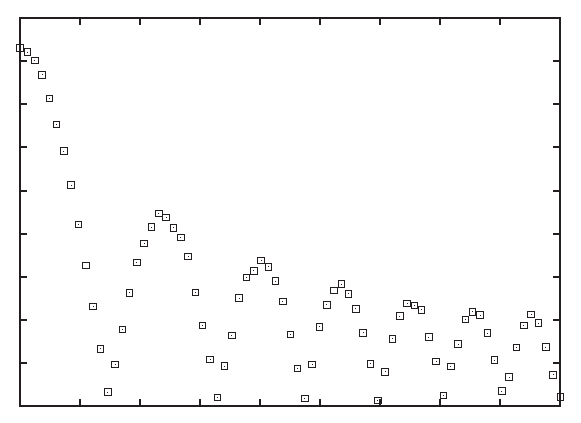
\includegraphics{img/bivariate1}}
  \caption{Data that clearly shows that there is a relationship,
    albeit a complicated one, between $x$ and $y$.}
  \label{fig:bivariate1}\vspace*{-6pt}
\end{figure}\pagebreak

In contrast, Figure \ref{fig:bivariate2} shows the kind of data
typical of much of statistical analysis. Here we might be showing the
prevalence of skin cancer as a function of the mean income for a group
of individuals or the unemployment rate as a function of the frequency
of high-school drop-outs for a number of counties, and the primary
question is whether there is any relationship at all between the two
quantities involved.  The situation here is quite different from that
shown in Figure \ref{fig:bivariate1}, where it was obvious that a
strong relationship existed between $x$ and $y$, and therefore our main
concern was to determine the precise nature of that relationship.

\begin{figure}
  \centerline{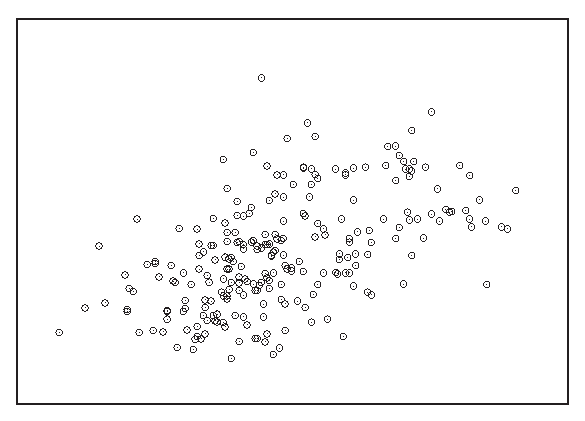
\includegraphics{img/bivariate2}}
  \caption{A noisy data set. Is there any relationship between $x$
    and $y$?}
  \label{fig:bivariate2}\vspace*{12pt}
\end{figure}

A figure such as Figure \ref{fig:bivariate2} is referred to as a
\emph{scatter plot} or \emph{xy plot}. I prefer the latter term
because scatter plot sounds to me too much like ``splatter plot,''
suggesting that the data necessarily will be noisy---but we don't know
that!  Once we plot the data, it may turn out to be very clean and
regular, as in Figure \ref{fig:bivariate1}; hence I am more
comfortable with the neutral term.

\begin{figure}[t!]
  \centerline{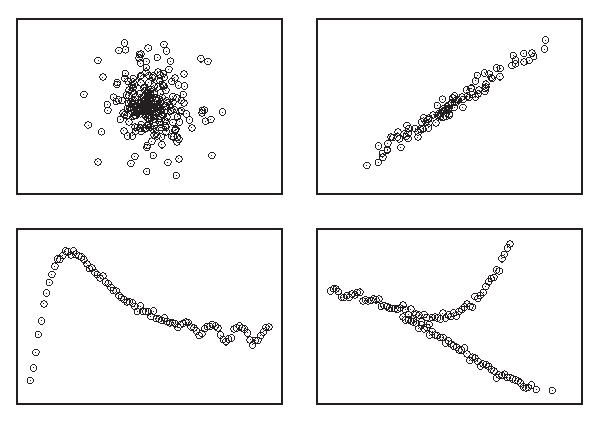
\includegraphics{img/bivariate3}}
  \caption{Four types of functional relationships (left to right, top
    to bottom): no relationship; strong, simple relationship; strong,
    not-simple relationship; multivariate relationship.}
  \label{fig:bivariate3}\vspace*{12pt}
\end{figure}

When we create a graph such as Figure \ref{fig:bivariate1} or Figure
\ref{fig:bivariate2}, we usually want to understand whether there is a
relationship between $x$ and $y$ as well as what the nature of that
relationship is. Figure \ref{fig:bivariate3} shows four different
possibilities that we may find: no relationship; a strong, simple
relationship; a strong, not-simple relationship; and finally a
multivariate relationship (one that is not unique).

% ============================================================
\section{Conquering Noise: Smoothing}

\index{bivariate analysis!noise and smoothing|(}
\index{noise|(}
\index{smoothing|(}
   
When data is noisy, we are more concerned with establishing
\emph{whether} the data exhibits a meaningful relationship, rather\vadjust{\pagebreak}
than establishing its precise character. To see this, it is often
helpful to find a smooth curve that represents the noisy data set.
Trends and structure of the data may be more easily visible from such
a curve than from the cloud of points.

Two different methods are frequently used to provide smooth
representation of noisy data sets: \emph{weighted splines}\index{weighted splines}\index{splines!weighted splines} and
a method known as \emph{LOESS} (or LOWESS), which is short for
locally weighted regression.

Both methods work by approximating the data in a small neighborhood
(\ie, locally) by a polynomial of low order (at most cubic). The trick
is to string the various local approximations together to form a
single smooth curve. Both methods contain an adjustable parameter that
controls the ``stiffness'' of the resulting curve: the stiffer the
curve, the smoother it appears but the less accurately it can follow
the individual data points. Striking the right balance between
smoothness and accuracy is the main challenge when it comes to
smoothing methods.

\spreadlong{-12pt}

\vspace*{-6pt}
\subsection{Splines}

\index{noise!splines}
\index{smoothing!splines}
\index{splines!about} 

Splines are constructed from piecewise polynomial functions \index{polynomials!splines} (typically
cubic) that are joined together in a smooth fashion. In addition to
the local smoothness requirements at each joint, splines must also
satisfy a global smoothness condition by optimizing the functional:\vspace*{-3pt}
%
\[
J[s] = \alpha \int \paren{ \diff[2]{s}{t} }^2 \rms{t}
     + (1-\alpha) \sum_i w_i \paren{ y_i - s(x_i) }^2\vspace*{-3pt}
\]
%
Here $s(t)$ is the spline curve, $(x_i, y_i)$ are the coordinates of
the data points, the $w_i$ are weight factors (one for each data
point), and $\alpha$ is a mixing factor. The first term controls how
``wiggly'' the spline is overall, because the second derivative
measures the curvature of $s(t)$ and becomes large if the curve has
many wiggles. The second term captures how accurately the spline
represents the data points by measuring the squared deviation of the
spline from each data point---it becomes large if the spline does not
pass close to the data points.  Each term in the sum is multiplied by
a weight factor $w_i$, which can be used to give greater weight to
data points that are known with greater accuracy than others. (Put
differently: we can write $w_i$ as $w_i = 1/d_i^2$, where $d_i$
measures how close the spline should pass by $y_i$ at $x_i$.) The
mixing parameter $\alpha$ controls how much weight we give to the
first term (emphasizing overall smoothness) relative to the second
term (emphasizing accuracy of representation).  In a plotting program,
$\alpha$ is usually the dial we use to tune the spline for a given
data set.

% Para below beautiful example of CE inadvertently and subtly changing 
% the semantics. ;-)
To construct the spline explicitly, we form cubic interpolation
polynomials for each consecutive pair of points and require that
these individual polynomials have the same values, as well as the same
first and second derivatives, at the points where they meet. These
smoothness conditions lead to a set of linear equations for the
coefficients in the polynomials, which can be solved. Once these
coefficients have been found, the spline curve can be evaluated at any
desired location.

\subsection{LOESS}

\index{noise!LOESS}
\index{smoothing!LOESS}
\index{LOESS!about|(}
  
Splines have an \emph{overall} smoothness goal, which means that they
are less responsive to \emph{local} details in the data set. The LOESS
smoothing method addresses this concern. It consists of approximating
the data locally through a low-order (typically linear) polynomial \index{polynomials!LOESS} 
(regression), \index{linear regression!LOESS} while weighting all the data points in such a way that
points close to the location of interest contribute more strongly than
do data points farther away (local weighting).

Let's consider the case of first-order (linear) LOESS, so that the local
approximation takes the particularly simple form $a + bx$. To find the
``best fit'' in a least-squares sense, we must minimize:
%
\[
\chi^2 = \sum_i w( x-x_i; h ) \paren{ a + b x_i - y_i }^2
\]
%
with respect to the two parameters $a$ and $b$. Here, $w(x)$ is the
weight function. It should be smooth and strongly peaked---in fact, it
is basically a kernel, similar to those we encountered in Figure
\ref{fig:kernels} when we discussed kernel density estimates.  The
kernel most often used with LOESS is the ``tri-cube'' kernel $K(x) =
\paren{ 1-|x|^3 }^3$ for $|x|<1$, $K(x)=0$ otherwise; but any of the
other kernels will also work.  The weight depends on the distance
between the point $x$ where we want to evaluate the LOESS
approximation and the location of the data points. In addition, the
weight function also depends on the parameter $h$, which controls the
bandwidth of the kernel: this is the primary control parameter for
LOESS approximations.  Finally, the value of the LOESS approximation
at position $x$ is given by $y(x) = a + b x$, where $a$ and $b$
minimize the expression for $\chi^2$ stated earlier.

This is the basic idea behind LOESS. You can see that it is easy to
generalize---for example, to two or more dimensions or two higher-order
approximation polynomials. (One problem, though: explicit, closed
expressions for the parameters $a$ and $b$ can be found only if you
use first-order polynomials; whereas for quadratic or higher
polynomials you will have to resort to numerical minimization
techniques. Unless you have truly compelling reasons, you want to
stick to the linear case!)

LOESS is a computationally intensive method. Keep in mind that the
entire calculation must be performed for \emph{every} point at which
we want to obtain a smoothed value. (In other words, the parameters
$a$ and $b$ that we calculated are themselves functions of $x$.) This
is in contrast to splines: once the spline coefficients have been
calculated, the spline can be evaluated easily at any point that we
wish. In this way, splines provide a summary or approximation to the
data. LOESS, however, does not lend itself easily to semi-analytical
work: what you see is pretty much all you get.

One final observation: if we replace the linear function $a + bx$ in
the fitting process with the constant function $a$, then LOESS becomes
simply a weighted moving average.

\subsection{Examples}

\index{noise!examples|(}
\index{smoothing!examples|(}

Let's look at two examples where smoothing reveals behavior that would
otherwise not be visible.

The first is a famous data set that has been analyzed in many places:
the 1970 draft lottery. \index{draft lottery, LEOSS} During the Vietnam War, men in the
U.S.\ were drafted based on their date of birth. Each possible birth date was
assigned a draft number between 1 and 366 using a lottery process, and
men were drafted in the order of their draft numbers. However,
complaints were soon raised that the lottery was biased---that men
born later in the year had a greater chance of receiving a low draft
number and, consequentially, a greater chance of being drafted
early.\footnote{More details and a description of the lottery process
  can be found in \cit{The Statistical Exorcist}{M.\ Hollander and F.\
    Proschan}{CRC Press}{1984}.}

\begin{figure}
\vspace*{-18pt}
  \centerline{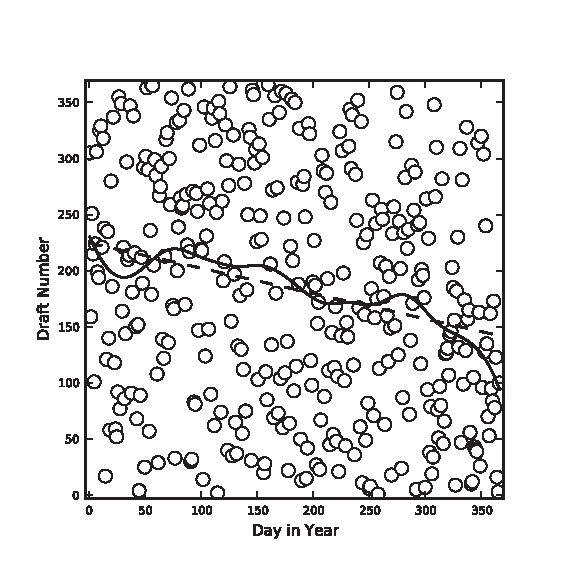
\includegraphics[scale=0.9]{img/draftlottery}}
  \caption{The 1970 draft lottery: draft number versus birth date (the
    latter as given in days since the beginning of the year).  Two
    LOESS curves with different values for the smoothing parameter $h$
    indicate that men born later in the year tended to have lower
    draft numbers. This would not be easily recognizable from a plot
    of the data points alone.}
  \label{fig:draftlottery}\vspace*{-6pt}
\end{figure}

Figure \ref{fig:draftlottery} shows all possible birth dates (as days
since the beginning of the year) and their assigned draft numbers.\vadjust{\pagebreak}  If
the lottery had been fair, these points should form a completely
random pattern. Looking at the data alone, it is virtually impossible
to tell whether there is any structure in the data. However, the
smoothed LOESS lines reveal a strong falling tendency of the draft
number over the course of the year: later birth dates are indeed more
likely to have a lower draft number!

The LOESS lines have been calculated using a Gaussian kernel. \index{Gaussian kernel, LOESS} For the
solid line, I used a kernel bandwidth equal to $5$, but for the dashed
line, I used a much larger bandwidth of $100$. For such a large
bandwidth, practically all points in the data set contribute equally
to the smoothed curve, so that the LOESS operation reverts to a linear
regression of the entire data set. (In other words: if we make the
bandwidth very large, then LOESS amounts to a least-squares fit of a
straight line to the data.)

In this draft number example, we mostly cared about a \emph{global}
property of the data: the presence or absence of an overall trend.
Because we were looking for a global property, a stiff curve (such as
a straight line) was sufficient to reveal what we were looking for.
However, if we want to extract more detail---in particular if we want
to extract \emph{local} features---then we need a ``softer'' curve,
which can follow the data on smaller scales.

Figure \ref{fig:marathon} shows an amusing example.\footnote{This
  example was inspired by \cit{Graphic Discovery: A Trout in the Milk
    and Other Visual Adventures}{Howard Wainer}{2nd ed., Princeton
    University Press}{2007}.} Displayed are the finishing times
(separately for men and women) for the winners in a marathon. Also
shown are the ``best fit'' straight-line approximations for all events
up to 1990. According to this (straight-line) model, women should
start finishing faster than men before the year 2000 and then continue
to become faster at a dramatic rate! This expectation is not borne out
by actual observations: finishing times for women (and men) have
largely leveled off.

\begin{figure}
    \centerline{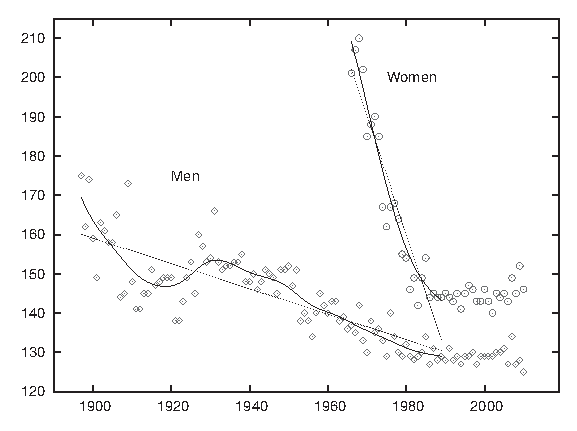
\includegraphics{img/marathon}}
  \caption{Winning times (in minutes) for an annual marathon event,
    separately for men and women. Also shown are the straight-line and
    smooth-curve approximations. All approximations are based entirely
    on data points \emph{prior} to 1990.}
  \label{fig:marathon}
\end{figure}

This example demonstrates the danger of attempting to describe data by
using a model of fixed form (a ``formula'')---and a straight line is
one of the most rigid models out there! A model that is not
appropriate for the data will lead to incorrect conclusions.
Moreover, it may not be obvious that the model is inappropriate. Look
again at Figure \ref{fig:marathon}: don't the straight lines seem
reasonable as a description of the data prior to 1990?

Also shown in Figure \ref{fig:marathon} are smoothed curves calculated
using a LOESS process. Because these curves are ``softer'' they have a
greater ability to capture features contained in the data.  Indeed,
the LOESS curve for the women's results does give an indication that
the trend of dramatic improvements, seen since they first started
competing in the mid-1960s, had already begun to level off before the
year 1990. (All curves are based strictly on data prior to 1990.) This
is a good example of how an adaptive smoothing curve can highlight
local behavior that is present in the data but may not be obvious
from merely looking at the individual data points.

\index{LOESS!about|)}
\index{noise!examples|)}
\index{smoothing!examples|)}

\subsection{Residuals}

\index{noise!residuals}
\index{smoothing!residuals}
\index{residuals, smoothing}

Once you have obtained a smoothed approximation to the data, you will
usually also want to check out the \emph{residuals}---that is, the
remainder when you subtract the smooth ``trend'' from the actual data.

There are several details to look for when studying residuals.

\begin{itemize}
\item Residuals should be balanced: symmetrically distributed around
  zero.
\item Residuals should be free of a trend. The presence of a trend or
  of any other large-scale systematic behavior in the residuals
  suggests that the model is inappropriate! (By construction, this is
  never a problem if the smooth curve was obtained from an adaptive
  smoothing model; however, it is an important indicator if the smooth
  curve comes from an analytic model.)
\item Residuals will necessarily straddle the zero value; they will
  take on both positive and negative values. Hence you may also want
  to plot their absolute values to evaluate whether the overall
  magnitude of the residuals is the same for the entire data set or
  not. The assumption that the magnitude of the variance around a
  model is constant throughout (``homoscedasticity'') \index{homoscedasticity, LOESS} is often an
  important condition in statistical methods. If it is not satisfied,
  then such methods may not apply.
\item Finally, you may want to use a QQ plot \index{QQ plots!LOESS} (see Chapter
  \ref{ch:univariate}) to check whether the residuals are distributed
  according to a Gaussian distribution. This, too, is an assumption
  that is often important for more advanced statistical methods.
\end{itemize}

It may also be useful to apply a smoothing routine to the
\emph{residuals} in order to recognize their features more clearly.
Figure \ref{fig:residuals} shows the residuals for the women's
marathon results (before 1990) both for the straight-line model and
the LOESS smoothing curve. For the LOESS curve, the residuals are
small overall and hardly exhibit any trend. For the straight-line
model, however, there is a strong systematic trend in the residuals
that is increasing in magnitude for years past 1985. This kind of
systematic trend in the residuals is a clear indicator that the model
is not appropriate for the data!

\begin{figure}
  \centerline{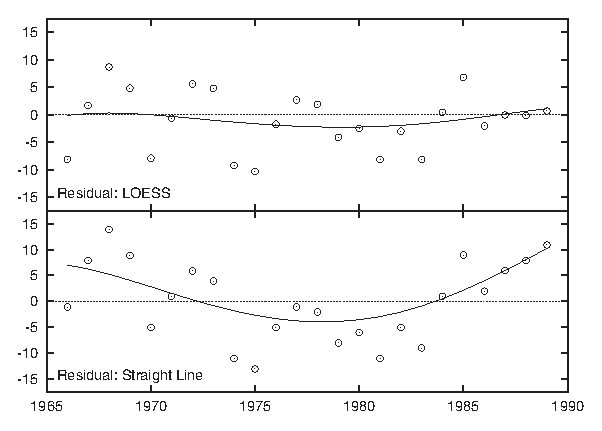
\includegraphics{img/residuals}}
  \caption{Residuals for the women's marathon results, both for the
    LOESS smoothing curve and the straight-line linear regression
    model. The residuals for the latter show an overall systematic
    trend, which suggests that the model does not appropriately
    describe the data.}
  \label{fig:residuals}
\end{figure}

\subsection{Additional Ideas and Warnings}

\index{noise!ideas and warnings}
\index{smoothing!ideas and warnings}

Here are some additional ideas that you might want to play with.

As we have discussed before, you can calculate the residuals between
the real data and the smoothed approximation. Here an isolated large
residual is certainly odd: it suggests that the corresponding data
point is somehow ``different'' than the other points in the
neighborhood---in other words, an outlier. Now we argue as follows.
If the data point is an outlier, then it should contribute less to the
smoothed curve than other points. Taking this consideration into
account, we now introduce an additional weight factor for each data
point into the expression for $J[s]$ or $\chi^2$ given previously.
The magnitude of this weight factor is chosen in such a way that data
points with large residuals contribute less to the smooth curve.  With
this new weight factor reducing the influence of points with large
residuals, we calculate a \emph{new} version of the smoothed
approximation. This process is iterated until the smooth curve no
longer changes.

Another idea is to split the original data points into two classes:
those that give rise to a positive residual and those with a negative
residual. Now calculate a smooth curve for each class separately. The
resulting curves can be interpreted as ``confidence bands'' for the
data set (meaning that the majority of points will lie between the
upper and the lower smooth curve). We are particularly interested to
see whether the width of this band varies along the curve. Figure
\ref{fig:smoothtube} shows an example that uses the men's results from
Figure \ref{fig:marathon}.

\begin{figure}
  \centerline{  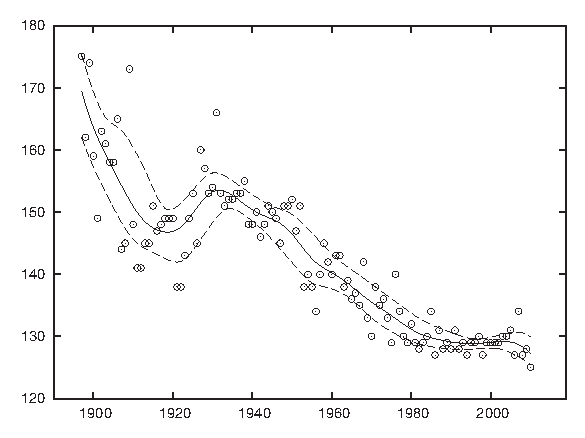
\includegraphics{img/smoothtube}}
  \caption{A ``smooth tube'' for the men's marathon results. The solid
    line is a smooth representation of the entire data set; the dashed
    lines are smooth representations of only those points that lie above
    (or below) the solid line.}
  \label{fig:smoothtube}
\end{figure}

Personally, I am a bit uncomfortable with either of these suggestions.
They certainly have an unpleasant air of circular reasoning about them.

There is also a deeper reason. \index{graphical analysis!interpretation} In my opinion, smoothing methods are a
quick and useful but entirely nonrigorous way to explore the structure
of a data set. With some of the more sophisticated extensions (\eg,
the two suggestions just discussed), we abandon the simplicity of the
approach without gaining anything in rigor! If we need or want better
(or deeper) results than simple graphical methods can give us, isn't
it time to consider a more rigorous toolset?

This is a concern that I have with many of the more sophisticated
graphical methods you will find discussed in the literature. Yes, we
certainly \emph{can} squeeze ever more information into a graph using
lines, colors, symbols, textures, and what have you. But this does not
necessarily mean that we \emph{should}. The primary benefit of a graph
is that it speaks to us directly---without the need for formal
training or long explanations. Graphs that require training or
complicated explanations to be properly understood are missing their
mark no matter how ``clever'' they may be otherwise.

Similar considerations apply to some of the more involved ways of
graph preparation. After all, a smooth curve such as a spline or LOESS
approximation is only a rough approximation to the data set---and, by
the way, contains a huge degree of arbitrariness in the form of the
smoothing parameter ($\alpha$ or $h$, respectively). Given this
situation, it is not clear to me that we need to worry about such
details as the effect of individual outliers on the curve.

Focusing too much on graphical methods may also lead us to miss the
essential point. For example, once we start worrying about confidence
bands, we should really start \emph{thinking more deeply} about the
nature of the local distribution of residuals (Are the residuals
normally distributed? Are they independent? Do we have a reason to
prefer one statistical model over another?)---and possibly consider a
more reliable estimation method (\eg, bootstrapping; see Chapter
\ref{ch:simulation})---rather than continue with hand-waving
(semi-)graphical methods.

Remember: The purpose of computing is insight, not pictures! (L.\ N.\
Trefethen)

\index{bivariate analysis!noise and smoothing|)}
\index{noise|)}
\index{smoothing|)}



% ============================================================
\section{Logarithmic Plots}

\index{bivariate analysis!logarithmic plots|(}
\index{logarithmic plots|(}
  
Logarithmic plots are a standard tool of scientists, engineers, and
stock analysts everywhere. They are so popular because they
have three valuable benefits:

\begin{itemize}
\item They rein in large variations in the data.
\item They turn multiplicative variations into additive ones.
\item They reveal exponential and power law behavior.
\end{itemize}

In a logarithmic plot, we graph the \emph{logarithm} of the data
instead of the raw data. Most plotting programs can do this for us (so
that we don't have to transform the data explicitly) and also take
care of labeling the axes appropriately.

There are two forms of logarithmic plots: \emph{single} or\index{single log plots}
\emph{semi-logarithmic} plots \index{semi-logarithmic plots} and \emph{double logarithmic} \index{double logarithmic plots} or
\emph{log-log} plots, \index{log-log plots} depending whether only one (usually the vertical
or $y$ axis) or both axes have been scaled logarithmically.

All logarithmic plots are based on the fundamental property of the
logarithm to turn products into sums and powers into products:
%
\begin{gather*}
  \log(x y) = \log(x) + \log(y) \\
  \log(x^k) = k \log(x)
\end{gather*}
%
Let's first consider semi-log plots. Imagine you have data generated
by evaluating the function:
%
\[
y = C \exp(\alpha x) \quad \text{where $C$ and $\alpha$ are constants}
\]
%
on a set of $x$ values. If you plot $y$ as a function of $x$, you will
see an upward- or downward-sloping curve, depending on the sign of
$\alpha$ (see Appendix \ref{app:calculus}). But if you instead plot
the \emph{logarithm} of $y$ as a function of $x$, the points will fall
on a straight line. This can be easily understood by applying the
logarithm to the preceding equation:
%
\[
\log y = \alpha x + \log C
\]
%
In other words, the logarithm of $y$ is a linear function of $x$ with
slope $\alpha$ and with offset $\log C$. In particular, by measuring
the slope of the line, we can determine the scale factor $\alpha$,
which is often of great interest in applications.

Figure \ref{fig:semilog} shows an example of a semi-logarithmic plot
that contains some experimental data points as well as an exponential
function for comparison. I'd like to point out a few details. First,
in a logarithmic plot, we plot the logarithm of the values, but the
axes are usually labeled with the actual values (not their
logarithms). Figure \ref{fig:semilog} shows both: the actual values on
the left and the logarithms on the right (the logarithm of 100 to base
10 is 2, the logarithm of 1,000 is 3, and so on). We can see how, in a
logarithmic plot, the logarithms are equidistant, but the actual values
are not. (Observe that the distance between consecutive tick marks is
constant on the right, but not on the left.)

\begin{figure}
  \centerline{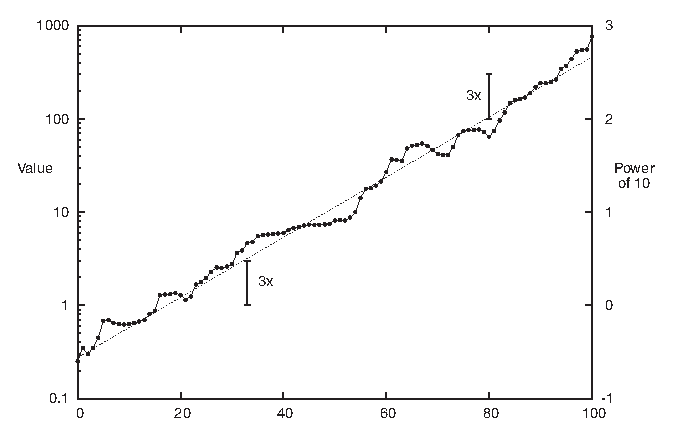
\includegraphics{img/semilog}}
  \caption{A semi-logarithmic plot.}
  \label{fig:semilog}
\end{figure}

Another aspect I want to point out is that on a semi-log plot, all
\emph{relative} changes have the same size no matter how large the
corresponding absolute change. It is this property that makes semi-log
plots popular for long-running stock charts and the like: if you lost
\$100, your reaction may be quite different if originally you had
invested \$1,000 versus \$200: in the first case you lost 10 percent
but 50 percent in the second. In other words, relative change is what
matters.

The two scale arrows in Figure \ref{fig:semilog} have the same length
and correspond to the same relative change, but the underlying
absolute change is quite different (from 1 to 3 in one case, from 100
to 300 in the other). This  is another application of the fundamental
property of the logarithm: if the value before the change is $y_1$ and
if $y_2 = \gamma y_1$ after the change (where $\gamma = 3$), then the
change in absolute terms is:
%
\[
y_2 - y_1 = \gamma y_1 - y_1 = (\gamma - 1) y_1
\]
%
which clearly depends on $y_1$. But if we consider the change
in the logarithms, we find:
%
\[
\log y_2 - \log y_1 
  = \log( \gamma y_1 ) - \log y_1 
  = \log \gamma + \log y_1 - \log y_1
  = \log \gamma
\]
%
which is independent of the underlying value and depends only
on $\gamma$, the size of the relative change.

\begin{figure}
  \centerline{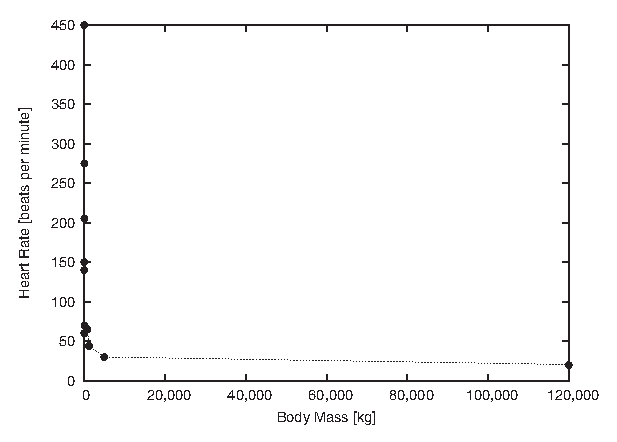
\includegraphics{img/allometric1}}\vspace*{-3pt}
  \caption{Heart rate versus body mass for a range of mammals. Compare
    to Figure \ref{fig:allometric2}.}
  \label{fig:allometric1}\vspace*{-6pt} 
\end{figure}

Double logarithmic plots \index{double logarithmic plots} are now easy to understand---the only
difference is that we plot logarithms of both $x$ \emph{and} $y$.
This will render all power-law relations as straight lines---that is,
as functions of the form $y = C x^k$ or $y = C/x^k$, where $C$ and $k$
are constants. (Taking logarithms on both sides of the first equation
yields $\log y = k \log x + \log C$, so that now $\log y$ is a linear
function of $\log x$ with a slope that depends on the exponent $k$.)

Figures \ref{fig:allometric1} and \ref{fig:allometric2} provide
stunning example for both uses of double logarithmic plots: their
ability to render data spanning many order of magnitude accessible and
their ability to reveal power-law relationships by turning them into
straight lines. Figure \ref{fig:allometric1} shows the typical resting
heart rate (in beats per minute) as a function of the body mass (in
kilograms) for a selection of mammals from the hamster to large 
whales. Whales weigh in at 120 tons---nothing else even comes close!
The consequence is that almost all of the data points are squished
against the lefthand side of the graph, literally crushed by the
whale.



On the double logarithmic plot, the distribution of data points
becomes much clearer. Moreover, we find that the data points are not
randomly distributed but instead seem to fall roughly on a straight
line with slope $-1/4$: the signature of power-law behavior. In other
words, a mammal's typical heart rate is related to its mass: larger
animals have slower heart beats. If we let $f$ denote the heart rate
and $m$ the mass, we can summarize this observation as:
%
\[
f \sim m^{-1/4}
\]

\begin{figure}
  \centerline{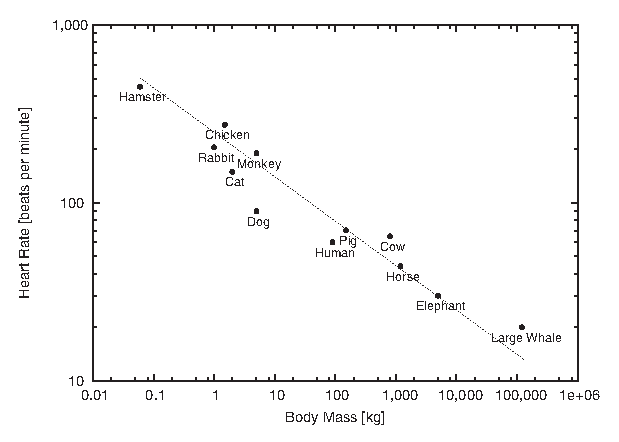
\includegraphics{img/allometric2}}
  \caption{The same data as in Figure \ref{fig:allometric1} but now
    plotted on a double logarithmic plot. The data points seem to fall
    on a straight line, which indicates a power-law relationship
    between resting heart rate and body mass.}
  \label{fig:allometric2} \vspace*{-6pt}
\end{figure}

This surprising result is known as \emph{allometric scaling}. \index{allometric scaling} It seems
to hold more generally and not just for the specific animals and
quantities shown in these figures. (For example, it turns out that the
lifetime of an individual organism also obeys a $1/4$ power-law
relationship with the body mass: larger animals live longer. The
surprising consequence is that the total number of heartbeats per life
of an individual is approximately constant for all species!)
Allometric scaling has been explained in terms of the geometric
constraints of the vascular network (veins and arteries), which brings
nutrients to the cells making up a biological system.  It is
sufficient to assume that the network must be a space-filling fractal,
that the capillaries where the actual exchange of nutrients takes
place are the same size in all animals, and that the overall energy
required for transport  through the  network is
minimized, to derive the power-law relationships observed experimentally!\footnote{The
original
  reference is \pcit{A General Model for the Origin of Allometric Scaling
  Laws in Biology}{\newline G.~B.\ West, J.\ H.\ Brown, and B.\ J.\
  Enquist}{Science}{276}{1997}{122} Additional references
  can be found on the Web.}  We'll have more to say about scaling laws
and their uses in Part \ref{part:analytics}.

% --- XXX : Here, I had the log-histo discussion, now removed. Reinstate?

\index{bivariate analysis!logarithmic plots|)}
\index{logarithmic plots|)}

% ============================================================

\setcounter{footnote}{1}
\section{Banking}

\index{bivariate analysis!banking|(}
\index{banking|(} 

Smoothing methods and logarithmic plots are both tools that help us 
recognize structure in a data set. Smoothing methods reduce noise, and
logarithmic plots help with data sets spanning many orders of
magnitude.

Banking (or ``banking to 45 degrees'') is another graphical method.
It is different than the preceding ones because it does not work on
the \emph{data} but on the plot as a whole by changing its aspect
ratio.

We can recognize \emph{change} (\ie, the slopes of curves) most
easily if they make approximately a 45 degree angle on the graph. It
is much harder to see change if the curves are nearly horizontal or
(even worse) nearly vertical. The idea behind \emph{banking} is
therefore to adjust the aspect ratio of the entire plot in such a way
that most slopes are at an approximate 45 degree angle. 

Chances are, you have been doing this already by changing the plot
\emph{ranges}. Often when we ``zoom'' in on a graph it's not so much
to see more detail as to adjust the slopes of curves to make them more
easily recognizable. The purpose is even more obvious when we zoom
\emph{out}. Banking is a more suitable technique to achieve the same
effect and opens up a way to control the appearance of a plot by
actively adjusting the aspect ratio.\index{aspect ratios, banking}

Figures \ref{fig:sunspot1} and \ref{fig:sunspot2} show the classical
example for this technique: the annual number of sunspots measured
over the last 300 years.\footnote{The discussion here is adapted from my
  book \emph{Gnuplot in Action}. Manning Publications. 2010.}  In
Figure \ref{fig:sunspot1}, the oscillation is very compressed, and so
it is difficult to make out much detail about the shape of the curve.
In Figure \ref{fig:sunspot2}, the aspect ratio of the plot has been
adjusted so that most line segments are now at roughly a 45 degree
angle, and we can make an interesting observation: the rising edge of
each sunspot cycle is steeper than the falling edge. We would probably
not have recognized this by looking at Figure \ref{fig:sunspot1}.

\begin{figure}
  \centerline{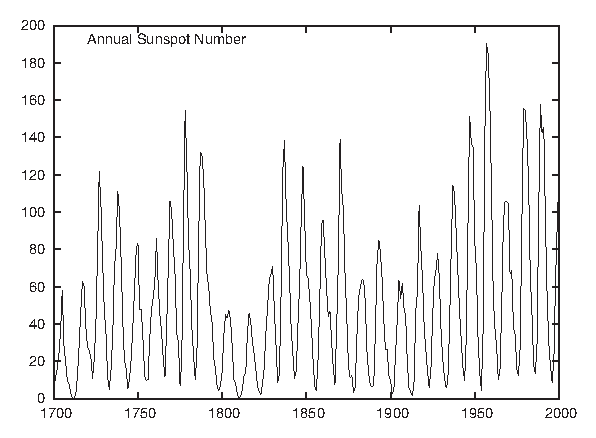
\includegraphics{img/sunspot1}}
  \caption{The annual sunspot numbers for the last 300 years. The
    aspect ratio of the plot makes it hard to recognize the details of
    each cycle.}
  \label{fig:sunspot1}%\vspace*{-12pt}
\end{figure}

\begin{figure}
  \centerline{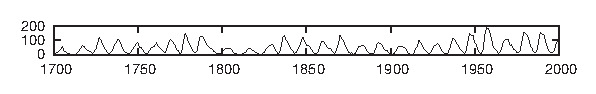
\includegraphics{img/sunspot2}}
  \caption{The same data as in Figure \ref{fig:sunspot1}. The aspect
    ratio has been changed so that rising and falling flanks of the
    curve make approximately a 45 degree angle with the horizontal
    (banking to 45 degrees), but the figure has become so small that
    it is hard to recognize much detail.}
  \label{fig:sunspot2}\vspace*{-6pt}
\end{figure} 

Personally, I would probably not use a graph such as Figure
\ref{fig:sunspot2}: shrinking the vertical axis down to almost nothing
loses too much detail. It also becomes difficult to compare the
behavior on the far left and far right of the graph. Instead, I would
break up the time series and plot it as a \emph{cut-and-stack plot},
such as the one in Figure \ref{fig:sunspot3}. Note that in this plot
the aspect ratio of each subplot is such that the lines are, in fact,
banked to 45 degrees.

As this example demonstrates, banking is a good technique but can be
taken too literally. When the aspect ratio required to achieve proper
banking is too skewed, it is usually better to rethink the entire
graph. No amount of banking will make the data set in 
Figure~\ref{fig:allometric1} look right---you need a double logarithmic
transform.

There is also another issue to consider.  The purpose of banking is to
improve human perception of the graph (it is, after all, exactly the\vadjust{\pagebreak}
same data that is displayed). But graphs with highly skewed aspect
ratios violate the great affinity humans seem to have for proportions
of roughly 4 by 3 (or 11 by 8.5 or $\sqrt{2}$ by $1$). Witness the
abundance of display formats (paper, books, screens) that adhere
approximately to these proportions the world over. Whether we favor
this display format because we are so used to it or (more likely, I
think) it is so predominant because it works well for humans is rather
irrelevant in this context. (And keep in mind that squares seem to
work particularly badly---notice how squares, when used for furniture
or appliances, are considered a ``bold'' design.  Unless there is a
good reason for them, such as graphing a square matrix, I recommend
you avoid square displays.)

\index{bivariate analysis!banking|)}
\index{banking|)} 

\begin{figure}
  \centerline{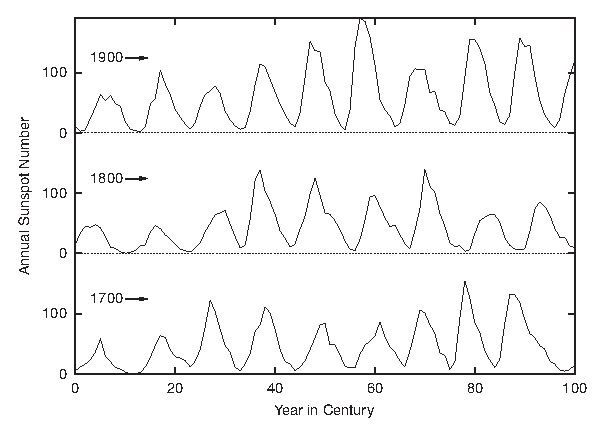
\includegraphics{img/sunspot3}}
  \caption{A cut-and-stack plot of the data from Figure
    \ref{fig:sunspot1}.  By breaking the time axis into three chunks,
    we can bank each century to 45 degrees and still fit all the data
    into a standard-size plot.  Note how we can now easily recognize
    an important feature of the data: the rising flank tends to be
    steeper than the falling one.}
  \label{fig:sunspot3}
\end{figure}

\vspace*{-6pt}
% ============================================================
\section{Linear Regression and All That}

\index{bivariate analysis!linear regression|(} 
\index{linear regression!about|(}
 
Linear regression is a method for finding a straight line through
a two-dimensional scatter plot. It is simple to calculate and
has considerable intuitive appeal---both of which together make
it easily the single most-often misapplied technique in all of
statistics!

There is a fundamental misconception regarding linear
regression---namely that it is a good and particularly rigorous way to
\emph{summarize}\vadjust{\pagebreak} the data in a two-dimensional scatter plot.  This
misconception is often associated with the notion that linear
regression provides the ``best fit'' to the data.

This is not so. Linear regression is not a particularly good way to 
summarize data, and it provides a ``best fit'' in a much more limited
sense than is generally realized. 

Linear regression applies to situations where we have a set of input
values (the controlled variable) and, for each of them, we measure an
output value (the response variable).  Now we are looking for a linear
function $f(x) = a + b x$ as a function of the controlled variable $x$
that reproduces the response with the least amount of error. The
result of a linear regression is therefore a function that minimizes
the error in the responses for a given set of inputs.

This is an important understanding: the purpose of a regression
procedure is not to \emph{summarize} the data---the purpose is to
obtain a function that allows us to \emph{predict} the value of the
response variable (which is affected by noise) that we expect for a
certain value of the input variable (which is assumed to be known
exactly).

\begin{figure}
  \centerline{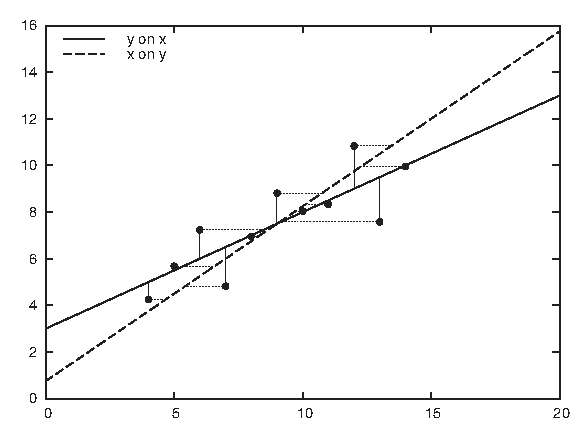
\includegraphics{img/regressionxy}}
  \caption{The first data set from Anscombe's quartet (Table
    \ref{tbl:anscombe}), fit both ways: $y = a + bx$ and $x = c + d
    y$. The thin lines indicate the errors, the squares of which are
    summed to give $\chi^2$. Depending on what you consider the input
    and the response variable, the ``best fit'' turns out to be
    different!}
  \label{fig:regressionxy}
\end{figure}

As you can see, there is a fundamental asymmetry between the two
variables: the two are not interchangeable.  In fact, you will obtain
a \emph{different} solution when you regress $x$ on $y$ than when you
regress $y$ on $x$. Figure \ref{fig:regressionxy} demonstrates this
effect: the same data set is fitted both ways: $y = a + bx$ and $x = c
+ d y$. The resulting straight lines are quite different.

This simple observation should dispel the notion that linear
regression provides \emph{the} best fit---after all, how could there
be two different ``best fits'' for a single\vadjust{\pagebreak} data set? Instead, linear
regression provides the most faithful representation of an output in
response to an input. In other words, \emph{linear regression is not
  so much a best fit as a best predictor}.

How do we find this ``best predictor''? We require it to minimize the
error in the responses, so that we will be able to make the most
accurate predictions.  But the error in the responses is simply the
sum over the errors for all the individual data points. Because errors
can be positive or negative (as the function over- or undershoots the
real value), they may cancel each other out. To avoid this, we do not sum
the errors themselves but their squares:
%
\begin{align*}
\chi^2 & = \sum_i \paren{ f(x_i) - y_i }^2 \\
       & = \sum_i \paren{ a + b x_i - y_i }^2
\end{align*}
%
where $(x_i, y_i)$ with $i=1 \dots n$ are the data points.  Using the
values for the parameters $a$ and $b$ that minimize this quantity will
yield a function that best explains $y$ in terms of $x$.

\begin{figure}
    \centerline{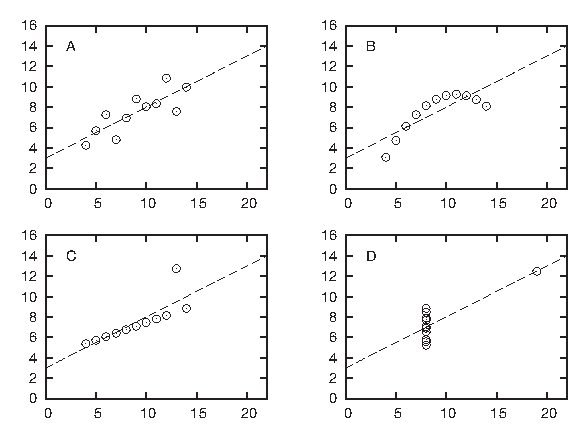
\includegraphics{img/anscombe}}
  \caption{Anscombe's quartet: all summary statistics (in particular
    the regression coefficients) for all four data sets are
    numerically equal, yet only data set A is well represented by the
    linear regression function.}
  \label{fig:anscombe}
\end{figure}

\begin{table}
\def\vrl{\smash{\vrule height124.5pt width.25pt depth3pt}}%
\def\vvrl{\smash{\vrule height138.5pt width.25pt depth3pt\hskip2pt\vrule height138.5pt width.25pt depth3pt}}%
\tbl{Anscombe's quartet.}{%
%\begin{center}
\begin{tabular}{@{\hskip6pt}r@{\hskip6pt}c@{\hskip-2pt}r@{\hskip6pt}c@{\hskip-2pt}r@{\hskip6pt}c@{\hskip-2pt}r@{\hskip6pt}c@{\hskip-2pt}r@{\hskip6pt}c@{\hskip-2pt}r@{\hskip6pt}c@{\hskip-2pt}r@{\hskip6pt}c@{\hskip-2pt}r@{\hskip6pt}}
\toprule
\multicolumn{2}{@{\hskip24pt}c@{\hskip-6pt}}{\TCH{A}} &&   \multicolumn{4}{c}{\TCH{B}} &&  \multicolumn{3}{c}{\TCH{C}} &&  \multicolumn{3}{c}{\TCH{D}} \\
\colrule
\multicolumn{1}{c}{\TCH{\itshape x}} & & \multicolumn{1}{c}{\TCH{\itshape y}} &&
\multicolumn{1}{c}{\TCH{\itshape x}} && \multicolumn{1}{c}{\TCH{\itshape y}} &&
\multicolumn{1}{c}{\TCH{\itshape x}} && \multicolumn{1}{c}{\TCH{\itshape y}} &&
\multicolumn{1}{c}{\TCH{\itshape x}} && \multicolumn{1}{c}{\TCH{\itshape y}} \\\colrule
10.0  && 8.04   && 10.0 && 9.14   && 10.0 && 7.46   && 8.0  && 6.58  \\ 
8.0   && 6.95   && 8.0  && 8.14   && 8.0  && 6.77   && 8.0  && 5.76  \\
13.0  && 7.58   && 13.0 && 8.74  && 13.0  && 12.74  && 8.0  && 7.71  \\
9.0   && 8.81   && 9.0  && 8.77   && 9.0  && 7.11   && 8.0  && 8.84  \\
11.0  && 8.33   && 11.0 && 9.26   && 11.0 && 7.81   && 8.0  && 8.47  \\
14.0  && 9.96   && 14.0 && 8.10   && 14.0 && 8.84   && 8.0  && 7.04  \\
6.0   && 7.24   && 6.0  && 6.13   && 6.0  && 6.08   && 8.0  && 5.25  \\
4.0   && 4.26   && 4.0  && 3.10   && 4.0  && 5.39   && 19.0 && 12.50 \\
12.0  && 10.84  && 12.0 && 9.13   && 12.0 && 8.15   && 8.0  && 5.56  \\
7.0   && 4.82   && 7.0  && 7.26   && 7.0  && 6.42   && 8.0  && 7.91  \\
5.0   &\vrl& 5.68   &\vvrl& 5.0  &\vrl& 4.74   &\vvrl& 5.0  &\vrl& 5.73   &\vvrl& 8.0  &\vrl& 6.89  \\
%\hline
\end{tabular}}\vspace*{6pt}
%\end{center} 
  \label{tbl:anscombe}
\end{table}

Because the dependence of $\chi^2$ on $a$ and $b$ is particularly
simple, we can work out expressions for the optimal choice of both
parameters explicitly. The results are:
%
\begin{gather*}
b = \frac{n \sum x_i y_i - \paren{\sum x_i} \paren{\sum y_i} }
         {n \paren{\sum x_i^2} - \paren{\sum x_i}^2 } \\
a = \frac{1}{n} \paren{\sum y_i - b \sum x_i}
\end{gather*}
%
These results are simple and beautiful---and, in their simplicity,
very suggestive. But they can also be highly misleading.  Table
\ref{tbl:anscombe} and Figure \ref{fig:anscombe} show a famous
example, \emph{Anscombe's quartet}. \index{Anscombe's Quartet} If you calculate the
regression coefficients $a$ and $b$ for each of the four data sets shown in Table
\ref{tbl:anscombe}, you will find that they are exactly the same for
all four data sets! Yet when you look at the corresponding scatter
plots, it is clear that only the first data set is properly described
by the linear model. The second data set is not linear, the third is
corrupted by an outlier, and the fourth does not contain enough
independent $x$ values to form a regression at all! Looking only at
the results of the linear regression, you would never know this.

 

I think this example should demonstrate once and for all how dangerous
it can be to rely on linear regression (or on any form of aggregate
statistics) to summarize a data set. (In fact, the situation is even
worse than what I have presented: with a little bit more work, you can
calculate confidence intervals on the linear regression results, and
even \emph{they} turn out to be equal for all four members of
Anscombe's quartet!)

Having seen this, here are some questions to ask \emph{before}
computing linear regressions.

\begin{unnumlist}
\subparagraph{Do you need regression?}
\item Remember that regression coefficients
  are not a particularly good way to \emph{summarize} data. Regression
  only makes sense when you want to use it for \emph{prediction}. If
  this is not the case, then calculating regression coefficients is not
  useful.

\subparagraph{Is the linear assumption appropriate?}
\item Linear regression is 
  appropriate only if the data can be described by a straight line.
  If this is obviously not the case (as with the second data set in
  Anscombe's quartet), then linear regression does not apply. 

\subparagraph{Is something else entirely going on?} 
\item
Linear regression,
  like all summary statistics, can be led astray by outliers or
  other ``weird'' data sets, as is demonstrated by the last two
  examples in Anscombe's quartet. 
\end{unnumlist}

Historically, one of the attractions of linear regression has been
that it is easy to calculate: all you need to do is to calculate the
four sums $\sum x_i$, $\sum x_i^2$, $\sum y_i$, and $\sum x_i y_i$,
which can be done in a single pass through the data set. Even with
moderately sized data sets (dozens of points), this is arguably easier
than plotting them using paper and pencil! However, that argument
simply does not hold anymore: graphs are easy to produce on a computer
and contain so much more information than a set of regression
coefficients that they should be the preferred way to analyze,
understand, and summarize data.

Remember: The purpose of computing is insight, not numbers! (R.\ W.\
Hamming)

\index{bivariate analysis!linear regression|)} 
\index{linear regression!about|)}
\vspace*{-9pt}
% ============================================================
\section{Showing What's Important}

\index{graphical analysis!process}

Perhaps this is a good time to express what I believe to be the most
important principle in graphical analysis:

% \emph{Show what you want to see!}
\emph{Plot the pertinent quantities!}

As obvious as it may appear, this principle is often overlooked in
practice.

For example, if you look through one of those books that show and
discuss examples of poor graphics, you will find that most examples
fall into one of two classes. First, there are those graphs that
failed \emph{visually}, with garish fonts, unhelpful symbols, and
useless embellishments. (These are mostly presentation graphics gone
wrong, not examples of bad graphical analysis.)

The second large class of graphical failures consists of those plots
that failed \emph{conceptually} or, one might better say,
\emph{analytically}. The problem\vadjust{\pagebreak} with these is not in the technical
aspects of drawing the graph but in the conceptual understanding of
what the graph is trying to show. These plots displayed something, but
they failed to present what was most important or relevant to the
question at hand.

The problem, of course, is that usually it is not at all obvious
\emph{what} we want to see, and it is certainly not obvious at the
beginning. It usually takes several iterations, while a mental model
of the data is forming in your head, to articulate the proper question
that a data set is suggesting and to come up with the best way of
answering it.  This typically involves some form of transformation or
manipulation of the data: instead of the raw data, maybe we should
show the difference between two data sets. Or the residual after
subtracting a trend or after subtracting the results from a model. Or
perhaps we need to normalize data sets from different sources by
subtracting their means and dividing by their spreads. Or maybe we
should not use the original variables to display the data but instead
apply some form of transformation on them (logarithmic scales are only
the simplest example of such transformations). Whatever we choose to
do, it will typically involve some form of transformation of the
data---it's rarely the raw data that is most interesting; but any
deviation from the expected is almost always an interesting discovery.

Very roughly, I think we can identify a three-step (maybe four-step)  
process. It should be taken not in the sense of a prescriptive
checklist but rather in the sense of a gradual process of learning and
discovery.

\paragraph{First: The basics.} Initially, we are mostly concerned with
displaying what is there.
\begin{itemize}
\item Select proper ranges.
\item Subtract a constant offset.
\item Decide whether to use symbols (for scattered data), lines (for
  continuous data), or perhaps both (connecting individual symbols
  can help emphasize trends in sparse data sets).
\end{itemize}

\paragraph{Second: The appearance.} Next, we work with aspects of the
plot that influence its overall appearance.
\begin{itemize}
\item Log plots.
\item Add a smoothed curve.
\item Consider banking.
\end{itemize}

\paragraph{Third: Build a model.} At this point, we start building a
mathematical model and compare it against the raw data. The comparison
often involves finding the differences between the model and the data
(typically subtracting the model or forming a ratio).
\begin{itemize}
\item Subtract a trend.
\item Form the ratio to a base value or baseline.
\item Rescale a set of curves to collapse them onto each other.
\end{itemize}

\paragraph{Fourth (for presentation graphics only): Add embellishments.} Embellishments 
and decorations (labels, arrows, special symbols, explanations, and so
on) can make a graph much more informative and self-explanatory.
However, they are intended for an audience beyond the actual creator
of the graph. You will rarely need them during the \emph{analysis}
phase, when you are trying to find out something new about the data
set, but they are an essential part when \emph{presenting} your
results. This step should only occur if you want to communicate your
results to a wider and more general audience.

% ============================================================
\section{Graphical Analysis and Presentation Graphics}

\index{graphical analysis!defined}
\index{presentation graphics, defined} 
 
I have used the terms \emph{graphical analysis} and \emph{presentation
  graphics} without explaining them properly. In short:

\begin{unnumlist}
\subparagraph{Graphical analysis}
\item Graphical analysis is an investigation of
  data using graphical methods. The purpose is the discovery of
  \emph{new} information about the underlying data set. In graphical
  analysis, the proper question to ask is often not known at the
  outset but is discovered as part of the analysis.

\subparagraph{Presentation graphics}
\item Presentation graphics are concerned with
  the communication of information and results that are \emph{already
    understood}. The discovery has been made, and now it needs to be
  communicated clearly.
\end{unnumlist}

The distinction between these two activities is important, because
they do require different techniques and yield different work products.

During the analysis process, convenience and ease of use are the
predominant concerns---any amount of polishing is too much! Nothing
should keep you from redrawing a graph, changing some aspect of it,
zooming in or out, applying transformations, and changing styles.
(When working with a data set I haven't seen before, I probably create
dozens of graphs within a few minutes---basically, ``looking at the
data from all angles.'')  At this stage, any form of embellishment
(labels, arrows, special symbols) is inappropriate---you know what you
are showing, and creating any form of decoration on the graph will
only make you more reluctant to throw the graph away and start over.

For presentation graphics, the opposite applies. Now you already
know the results, but you would like to communicate them to others.
Textual information therefore becomes very important: how else will
people know what they are looking at?

You can find plenty of advice elsewhere on how to prepare ``good''
presentation graphics---often strongly worded and   with an
unfortunate tendency to use emotional responses (ridicule or derision)
in place of factual arguments.  In the absence of good empirical
evidence one way or the other, I will not add to the discussion. But I
present a \emph{checklist} below, mentioning some points that are
often overlooked when preparing graphs for presentation:
\begin{itemize}
\item Try to make the text self-explanatory. Don't rely on a (separate)
  caption for basic information---it might be removed during 
  reproduction. Place basic information on the graph itself.

\item Explain what is plotted on the axes. This can be done with 
  explicit labels on the axes or through explanatory text elsewhere.
  Don't forget the units!

\item Make labels self-explanatory. Be careful with nonstandard
  abbreviations. Ask yourself: If this is all the context provided,
  are you \emph{certain} that the reader will be able to figure out
  what you mean? (In a recent book on data graphing, I found a
  histogram labeled \emph{Married}, \emph{Nvd}, \emph{Dvd},
  \emph{Spd}, and \emph{Wdd}. I could figure out most of them, because
  at least \emph{Married} was given in long form, but I struggled with
  \emph{Nvd} for quite a while!)

\item Given how important \emph{text} is on a graph, make sure to pick
  a suitable font. Don't automatically rely on the default provided by
  your plotting software. Generally, sans-serif fonts (such as
  Helvetica) are preferred for short labels, such as those on a graph,
  whereas serif fonts (such as Times) are more suitable for body text.
  Also pick an appropriate size---text fonts on graphics are often too
  large, making them look garish. (Most text fonts are used at
  10-point to 12-point size; there is no need for type on graphics to
  be much larger.)

\item If there are error bars, be sure to explain their meaning. What
  are they: standard deviations, inter-quartile ranges, or the limits
  of experimental apparatus? Also, choose an appropriate measure of
  uncertainty. Don't use standard deviations for highly skewed data.

\item Don't forget the basics. Choose appropriate plot ranges. Make
  sure that data is not unnecessarily obscured by labels.

\item Proofread graphs! Common errors include: typos in textual
  labels, interchanged data sets or switched labels, missing units,
  and incorrect order-of-magnitude qualifiers (\eg, milli- versus
  micro-).

\item Finally, choose an appropriate output format for your graph!
  Don't use bitmap formats (GIF, JPG, PNG) for print publication---use
  a scalable format such as PostScript or PDF.
\end{itemize}

One last piece of advice: creating good presentation graphics is also
a matter of \emph{taste}, and taste can be acquired. If you want to
work with data, then you should develop an interest in graphs---not
just the ones you create yourself, but all that you see. If you notice
one that seems to work (or not), take a moment to figure out what
makes it so. Are the lines too thick? The labels too small? The choice
of colors just right? The combination of curves helpful? Details
matter.

% ============================================================
\section{Workshop: matplotlib}

\index{bivariate analysis!matplotlib|(}
\index{matplotlib|(}
  
The matplotlib module is a Python module for creating two-dimensional
$xy$ plots, scatter plots, and other plots typical of scientific
applications. It can be\vadjust{\pagebreak} used in an interactive session (with the plots
being shown immediately in a GUI window) or from within a script to
create graphics files using common graphics file formats.

Let's first look at some examples to demonstrate how matplotlib can be
used from within an interactive session. Afterward, we will take a
closer look at the structure of the library and give some pointers for
more detailed investigations.

\subsection{Using matplotlib Interactively}

\index{matplotlib!using interactively|(}
 
To begin an interactive matplotlib session, start IPython (the enhanced
interactive Python shell) with the \texttt{-pylab} option, entering
the following command line like at the shell prompt:

\begin{verbatim}
ipython -pylab  
\end{verbatim}

This will start IPython, load matplotlib \emph{and} NumPy, and import
both into the global namespace. The idea is to give a Matlab-like
experience of interactive graphics together with numerical and matrix
operations.  (It is important to use IPython here---the flow of
control between the Python command interpreter and the GUI eventloop
for the graphics windows requires it. Other interactive shells can be
used, but they may require some tinkering.)

We can now create plots right away:

\begin{verbatim}
In [1]: x = linspace( 0, 10, 100 )

In [2]: plot( x, sin(x) )
Out[2]: [<matplotlib.lines.Line2D object at 0x1cfefd0>]
\end{verbatim}

This will pop up a new window, showing a graph like the one in Figure
\ref{fig:mplt1} but decorated with some GUI buttons. (Note that the
\texttt{sin()} function is a ufunc from the NumPy package: it takes a
vector and returns a vector of the same size, having applied the sine
function to each element in the input vector. See the Workshop in
Chapter \ref{ch:univariate}.)

\begin{figure}
  \centerline{ 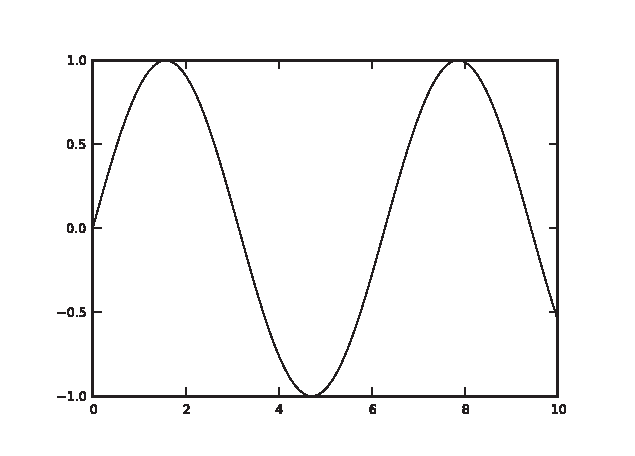
\includegraphics{img/mplt1}}
  \caption{A simple matplotlib figure (see text).}
  \label{fig:mplt1}
\end{figure}

We can now add additional curves and decorations to the plot. Continuing
in the same session as before, we add another curve and some labels:

\begin{verbatim}
In [3]: plot( x, 0.5*cos(2*x) )
Out[3]: [<matplotlib.lines.Line2D object at 0x1cee8d0>]

In [4]: title( "A matplotlib plot" )
Out[4]: <matplotlib.text.Text object at 0x1cf6950>

In [5]: text( 1, -0.8, "A text label" )
Out[5]: <matplotlib.text.Text object at 0x1f59250>

In [6]: ylim( -1.1, 1.1 )
Out[6]: (-1.1000000000000001, 1.1000000000000001)
\end{verbatim}

In the last step, we increased the range of values plotted on the
vertical axis. (There is also an \texttt{axis()} command, which allows
you to specify limits for both axes at the same time. Don't confuse it
with the \texttt{axes()} command, which creates a new coordinate
system.) The plot should now look like the one in Figure
\ref{fig:mplt2}, except that in an interactive terminal the different
lines are distinguished by their color, not their dash pattern.



% not really interactive - limits get reset!

Let's pause for a moment and point out a few details. First of all,
you should have noticed that the graph in the plot window was updated
after every operation. That is typical for the interactive mode, but it
is not how matplotlib works in a script: in general, matplotlib tries
to delay the (possibly expensive) creation of an actual plot until the
last possible moment. (In a script, you would use the \texttt{show()}
command to force generation of an actual plot window.)


\begin{figure}
   \centerline{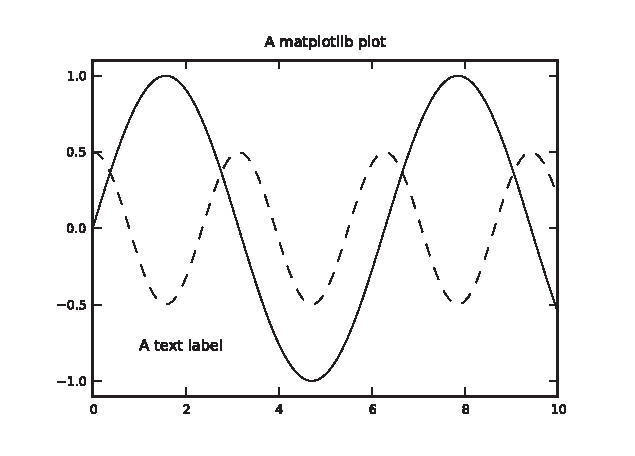
\includegraphics{img/mplt2}}
  \caption{The plot from Figure \ref{fig:mplt1} with an additional
    curve and some decorations added.}
  \label{fig:mplt2}\vspace*{-18pt}
\end{figure}

Furthermore, matplotlib is ``stateful'': a new plot command does not
erase the previous figure and, instead, adds to it. This behavior can
be toggled with the \texttt{hold()} command, and the current state can
be queried using \texttt{ishold()}. (Decorations like the text labels
are not affected by this.) You can clear a figure explicitly using
\texttt{clf()}.

This implicit state may come as a surprise: haven't we learned to make
things explicit, when possible? In fact, this stateful behavior is a
holdover from the way Matlab works. Here is another example. Start a
new session and execute the following commands:

\begin{verbatim}
In [1]: x1 = linspace( 0, 10, 40 )

In [2]: plot( x1, sqrt(x1), 'k-' )
Out[2]: [<matplotlib.lines.Line2D object at 0x1cfef50>]
\end{verbatim}

\begin{verbatim}
In [3]: figure(2)
Out[3]: <matplotlib.figure.Figure object at 0x1cee850>

In [4]: x2 = linspace( 0, 10, 100 )

In [5]: plot( x1, sin(x1), 'k--', x2, 0.2*cos(3*x2), 'k:' )
Out[5]: 
[<matplotlib.lines.Line2D object at 0x1fb1150>,
 <matplotlib.lines.Line2D object at 0x1fba250>]

In [6]: figure(1)
Out[6]: <matplotlib.figure.Figure object at 0x1cee210>

In [7]: plot( x1, 3*exp(-x1/2), linestyle='None', color='white', marker='o', 
   ...: markersize=7 )
Out[7]: [<matplotlib.lines.Line2D object at 0x1d0c150>]

In [8]: savefig( 'graph1.png' )
\end{verbatim}

This snippet of code demonstrates several things. We begin as before,
by creating a plot. This time, however, we pass a third argument to
the \texttt{plot()} command that controls the appearance of the graph
elements. That matplotlib library supports Matlab-style mnemonics for
plot styles; the letter \texttt{k} stands for the color ``black'' and
the single dash \texttt{-} for a solid line. (The letter \texttt{b}
stands for ``blue.'')

Next we create a second figure in a new window and switch to it by
using the \texttt{figure(2)} command. All graphics commands will now
be directed to this second figure---until we switch back to the
first figure using \texttt{figure(1)}. This is another example of
``silent state.'' Observe also that figures are counted starting from 1,
not from 0.

In line 5, we see another way to use the plot command---namely, by
specifying two sets of curves to be plotted together. (The formatting
commands request a dashed and a dotted line, respectively.) Line 7
shows yet a different way to specify plot styles: by using named
(keyword) arguments.

Finally, we save the currently active plot (\ie, figure 1) to a
PNG file. The \texttt{savefig()} function determines the desired
output format from the extension of the filename given. Other formats
that are supported out of the box are PostScript, PDF, and SVG.
Additional formats may be available, depending on the libraries
installed on your system.

\index{matplotlib!using interactively|)}

\subsection{Case Study: LOESS with matplotlib}
\index{matplotlib!LOESS case study}
\index{LOESS!matplotlib case study}  
As a quick example of how to put the different aspects of matplotlib
together, let's discuss the script used to generate Figure
\ref{fig:draftlottery}. This also gives us an opportunity to look at
the LOESS method in a bit more detail.

To recap: LOESS stands for \emph{locally weighted} linear regression.\index{linear regression!LOESS}
The difference between LOESS and regular linear regression is the introduction of a 
weight factor, which emphasizes those data points that are close to
the location $x$ at which we want to evaluate the smoothed curve. As
explained earlier, the expression for squared error (which we want to
minimize) now becomes:
%
\[
\chi^2(x) = \sum_i w( x-x_i; h ) \paren{ a + b x_i - y_i }^2
\]
%
Keep in mind that this expression now depends on $x$, the location
at which we want to evaluate the smoothed curve!

If we minimize this expression with respect to the parameters $a$ and
$b$, we obtain the following expressions for $a$ and $b$ (remember
that we will have to evaluate them from scratch for every point $x$):
\begin{gather*}
b = \frac{\sum w_i \sum w_i x_i y_i 
          - \paren{\sum w_i x_i} \paren{\sum w_i y_i} }
         {\sum w_i \paren{\sum w_i x_i^2} - \paren{\sum w_i x_i}^2 } \\
a = \frac{\paren{\sum w_i y_i - b \sum w_i x_i}}{\sum w_i}
\end{gather*}

This can be quite easily translated into NumPy and plotted with
matplotlib. The actual LOESS calculation is contained entirely in the
function \texttt{loess()}.  (See the Workshop in Chapter
\ref{ch:univariate} for a discussion of this type of programming.)\vspace*{6pt}

\begin{verbatim}
from pylab import *

# x: location; h: bandwidth; xp, yp: data points (vectors)
def loess( x, h, xp, yp ):
    w = exp( -0.5*( ((x-xp)/h)**2 )/sqrt(2*pi*h**2) )

    b = sum(w*xp)*sum(w*yp) - sum(w)*sum(w*xp*yp)
\end{verbatim}

\begin{verbatim}
    b /= sum(w*xp)**2 - sum(w)*sum(w*xp**2)
    a = ( sum(w*yp) - b*sum(w*xp) )/sum(w)

    return a + b*x

d = loadtxt( "draftlottery" )

s1, s2 = [], []
for k in d[:,0]:
    s1.append( loess( k,   5, d[:,0], d[:,1] ) )
    s2.append( loess( k, 100, d[:,0], d[:,1] ) )

xlabel( "Day in Year" )
ylabel( "Draft Number" )

gca().set_aspect( 'equal' )

plot( d[:,0], d[:,1], 'o', color="white", markersize=7, linewidth=3 )
plot( d[:,0], array(s1), 'k-', d[:,0], array(s2), 'k--' )

q = 4
axis( [1-q, 366+q, 1-q, 366+q] )

savefig( "draftlottery.eps" )
\end{verbatim}

We evaluate the smoothed curve at the locations of all data points,
using two different values for the bandwidth, and then proceed to plot
the data together with the smoothed curves. Two details require an
additional word of explanation.  The function \texttt{gca()} returns
the current ``set of axes'' (\ie, the current coordinate system on the
plot---see below for more information on this function), and we
require the aspect ratio of both $x$ and $y$ axes to be equal (so that
the plot is a square). In the last command before we save the figure
to file, we adjust the plot range by using the \texttt{axis()}
command. This function must \emph{follow} the \texttt{plot()}
commands, because the \texttt{plot()} command automatically adjusts
the plot range depending on the data.\vspace*{-18pt}

\subsection{Managing Properties}
\index{matplotlib!properties|(} 
Until now, we have ignored the values returned by the various plotting
commands. If you look at the output generated by IPython, you can see
that all the commands that add graph elements to the plot return a
reference to the object just created. The one exception is the
\texttt{plot()} command \index{plot command (matplotlib)} itself, which always returns a \emph{list} of
objects (because, as we have seen, it can add more than one ``line''
to the plot). 

These references are important because it is through them that we can
control the appearance of graph elements once they have been created.
In a final example, let's study how we can use them:

\begin{verbatim}
In [1]: x = linspace( 0, 10, 100 )

In [2]: ps = plot( x, sin(x), x, cos(x) )
\end{verbatim}

\begin{verbatim}
In [3]: t1 = text( 1, -0.5, "Hello" )

In [4]: t2 = text( 3, 0.5, "Hello again" )

In [5]: t1.set_position( [7, -0.5] )

In [6]: t2.set( position=[5, 0], text="Goodbye" )
Out[6]: [None, None]

In [7]: draw()

In [8]: setp( [t1, t2], fontsize=10 )
Out[8]: [None, None]

In [9]: t2.remove()

In [10]: Artist.remove( ps[1] )

In [11]: draw()
\end{verbatim} 

In the first four lines, we create a graph with two curves and two
text labels, as before, but now we are holding on to the object
references. This allows us to make changes to these graph elements.
Lines 5, 6, and 8 demonstrate different ways to do this: for each
property of a graph element, there is an explicit, named accessor
function (line 5). Alternatively, we can use a generic setter with
keyword arguments---this allows us to set several properties (on a
single object) in a single call (line 6). Finally, we can use the
standalone \texttt{setp()} function, \index{setp() function} which takes a list of graph
elements and applies the requested property update to all of them.
(It can also take a single graph element instead of a one-member
list.) Notice that \texttt{setp()} generates a redraw event whereas
individual property accessors do not; this is why we must generate an
explicit redraw event in line 7. (If you are confused by the apparent
duplication of functionality, read on: we will come back to this point
in the next section.)

Finally, we remove one of the text labels and one of the curves by
using the \texttt{remove()} function. \index{remove() function} The \texttt{remove()} function
is defined for objects that are derived from the \texttt{Artist}
class, so we can invoke it using either member syntax (as a ``bound''
function, line 9) or the class syntax (as an ``unbound'' function,
line 10). Keep in mind that \texttt{plot()} returns a \emph{list} of
objects, so we need to index into the list to access the graph objects
themselves.

There are some useful functions that can help us handle object
properties. If you issue \texttt{setp(r)} \index{setp() function} with only a single argument
in an interactive session, then it will print all properties that are
available for object  \texttt{r} together with information about the
values that each property is allowed to take on. The \texttt{getp(r)}
function \index{getp(r) function} on the other hand prints all properties of \texttt{r}
together with their current values.

% mixed functional/object stuff

Suppose we did not save the references to the objects we created, or
suppose we want to change the properties of an object that we did not
create explicitly. In such cases we can use the functions
\texttt{gcf()} \index{gcf() and gca() functions} and \texttt{gca()}, which return a\vadjust{\pagebreak} reference to the
current figure or axes object, respectively. To make use of them, we
need to develop at least a passing familiarity with matplotlib's
object model. 

\index{matplotlib!properties|)}

\subsection{The matplotlib Object Model and Architecture}

\index{matplotlib!object model and architecture}
\index{object model, matplotlib}
  
% http://matplotlib.sourceforge.net/leftwich_tut.txt

The object model for matplotlib is constructed similarly to the object
model for a GUI widget set: a plot is represented by a tree of
widgets, and each widget is able to render itself.  Perhaps
surprisingly, the object model is not flat. In other words, the plot
elements (such as axes, labels, arrows, and so on) are not properties
of a high-level ``plot'' or ``figure'' object. Instead, you must
descend down the object tree to find the element that you want to
modify and then, once you have an explicit reference to it, change the
appropriate property on the element.

The top-level element (the root node of the tree) is an object of
class \texttt{Figure}. A figure contains one or more \texttt{Axes}
objects: this class represents a ``coordinate system'' on which actual
graph elements can be placed. (By contrast, the actual axes that are
drawn on the graph are objects of the \texttt{Axis} class!) The
\texttt{gcf()} and \texttt{gca()} functions therefore return a
reference to the root node of the entire figure or to the root node of
a single plot in a multiplot figure.

Both \texttt{Figure} and \texttt{Axes} are subclasses of
\texttt{Artist}.  This is the base class of all ``widgets'' that can
be drawn onto a graph. Other important subclasses of \texttt{Artist}
are \texttt{Line2D} (a polygonal line connecting multiple points,
optionally with a symbol at each point), \texttt{Text}, and
\texttt{Patch} (a geometric shape that can be placed onto the figure).
The top-level \texttt{Figure} instance is owned by an object of type
\texttt{FigureCanvas} (in the \texttt{matplotlib.backend\_bases}
module). Most likely you won't have to interact with this class
yourself directly, but it provides the bridge between the (logical)
object tree that makes up the graph and a backend, which does the
actual rendering. Depending on the backend, matplotlib creates either
a file or a graph window that can be used in an interactive GUI
session.

% As you have seen, matplotlib is easy to use. It is not so easy to
% understand --- at least if you really want to get your arms around it.

Although it is easy to get started with matplotlib from within an
interactive session, it can be quite challenging to really get one's
arms around the whole library. This can become painfully clear when
you want to change some tiny aspect of a plot---and can't figure out
how to do that. 

As is so often the case, it helps to investigate how things came to
be. Originally, matplotlib was conceived as a plotting library to
emulate the behavior found in Matlab. Matlab traditionally uses a
programming  model based on functions and, being 30 years old, employs
some conventions that are no longer popular (\ie, implicit state).  In
contrast, matplotlib was implemented using object-oriented design
principles in Python, with the result that these two different
paradigms clash.

One consequence of having these two different paradigms side by side
is redundancy.  Many operations can be performed in several different
ways (using standalone functions, Python-style keyword arguments,
object attributes,\vadjust{\pagebreak} or a Matlab-compatible alternative syntax). We saw
examples of this redundancy in the third listing when we changed
object properties. This duplication of functionality matters because
it drastically increases the size of the library's interface (its
application programming interface or API), which makes it that much
harder to develop a comprehensive understanding.  What is worse, it
tends to spread information around. (Where should I be looking for
plot attributes---among functions, among members, among keyword
attributes? Answer: everywhere!)

Another consequence is inconsistency. At least in its favored
function-based interface, matplotlib uses some conventions that are
rather unusual for Python\index{Python!matplotlib}\index{software!Python} programming---for instance, the way a figure
is created \emph{implicitly} at the beginning of every example, and
how the pointer to the current figure is maintained through an
invisible ``state variable'' that is opaquely manipulated using the
\texttt{figure()} function. (The \texttt{figure()} function actually
returns the figure object just created, so the invisible state
variable is not even necessary.) Similar surprises can be found
throughout the library.
% Although the interface is function based, all functions return 
% members of the object model!

A last problem is namespace pollution (this is another Matlab
heritage---they didn't have namespaces back then).  Several
operations included in matplotlib's function-based interface are not
actually graphics related but do generate plots as \emph{side
  effects}. For example, \texttt{hist()} calculates (and plots) a
histogram, \texttt{acorr()} calculates (and plots) an autocorrelation
function, and so on. From a user's perspective, it makes more sense to
adhere to a separation of tasks: perform all calculations in
NumPy/SciPy, and then pass the results explicitly to matplotlib for
plotting.

\subsection{Odds and Ends}

There are three different ways to import and use matplotlib. The 
original method was to enter:

\begin{verbatim}
from pylab import *
\end{verbatim}

This would load all of NumPy\index{NumPy}\index{software!NumPy} as well as matplotlib and import both
APIs into the global namespace! This is no longer the preferred way to
use matplotlib. Only for interactive use with IPython is it still
required (using the \texttt{-pylab} command-line option to IPython).

The recommended way to import matplotlib's function-based interface
together with NumPy is by using:

\begin{verbatim}
import matplotlib.pyplot as plt
import numpy as np
\end{verbatim}

The \texttt{pyplot} \index{pyplot} interface is a function-based interface that uses
the same Matlab-like stateful conventions that we have seen in the
examples of this section; however, it does \emph{not} include the
NumPy functions.  Instead, NumPy must be imported separately (and into
its own namespace).

Finally, if all you want is the object-oriented API to matplotlib,
then you can import just the explicit modules from within matplotlib
that contain\vadjust{\pagebreak} the class definitions you need (although it is customary
to import \texttt{pyplot} instead and thereby obtain access to the
whole collection).

Of course, there are many details that we have not discussed. Let me
mention just a few: 

\begin{itemize}
\item Many more options (to configure the axes and tick marks, to add
   legend or arrows).
\item Additional plot types (density or ``false-color'' plots, vector
  plots, polar plots).
\item Digital image processing---matplotlib can read and manipulate PNG
  images and can also call into the Python Image Library (PIL) if
  it is installed.
\item Matplotlib can be embedded in a GUI and can handle GUI events.
\end{itemize}

The Workshop of Chapter \ref{ch:timeseries} contains another example
that involves matplotlib being called from a script to generate image
files.

\index{bivariate analysis!matplotlib|)}
\index{matplotlib|)}

% ============================================================
\section{Further Reading}

In addition to the books listed below, you may check the references
in Chapter \ref{ch:statistics} for additional material on linear
regression.

\begin{itemize}

\item \cit{The Elements of Graphing Data}{William S.\ Cleveland}{2nd ed.,
    Hobart Press}{1994}
  This is probably the definitive reference on graphical analysis (as
  opposed to presentation graphics). Cleveland is the inventor of both
  the LOESS and the banking techniques discussed in this chapter. My
  own thinking has been influenced strongly by Cleveland's careful
  approach.  A companion volume by the same author, entitled
  \emph{Visualizing Data}, is also available.
\item \cit{Exploratory Data Analysis with MATLAB}{Wendy L.\ Martinez
    and Angel R.\ Martinez}{Chapman \& Hall/CRC}{2004}
  This is an interesting book---it covers almost the same topics as
  the book you are reading but in \emph{opposite} order, starting with
  dimensionality reduction and clustering techniques and ending with
  univariate distributions! Because it demonstrates all techniques by
  way of Matlab, it does not develop the conceptual background in
  great depth. However, I found the chapter on smoothing to be quite
  useful.
\end{itemize}

\index{data analysis!bivariate analysis|)}
\index{bivariate analysis|)}
